% -*- coding: utf-8 -*-
%-------------------------designed by zcf--------------
\documentclass[UTF8,a4paper,10pt]{ctexrep}
\usepackage[left=3.17cm, right=3.17cm, top=2.74cm, bottom=2.74cm]{geometry}
\usepackage{amsmath}
\usepackage{graphicx,subfig}
\usepackage{float}
\usepackage{cite}
\usepackage{caption}
\usepackage{enumerate}
\usepackage{booktabs} %表格
\usepackage{multirow}
\newcommand{\tabincell}[2]{\begin{tabular}{@{}#1@{}}#2\end{tabular}}  %表格强制换行
%-------------------------字体设置--------------
% \usepackage{times} 
\usepackage{ctex}
\setCJKmainfont[ItalicFont=Noto Sans CJK SC Bold, BoldFont=Noto Serif CJK SC Black]{Noto Serif CJK SC}
\newcommand{\yihao}{\fontsize{26pt}{36pt}\selectfont}           % 一号, 1.4 倍行距
\newcommand{\erhao}{\fontsize{22pt}{28pt}\selectfont}          % 二号, 1.25倍行距
\newcommand{\xiaoer}{\fontsize{18pt}{18pt}\selectfont}          % 小二, 单倍行距
\newcommand{\sanhao}{\fontsize{16pt}{24pt}\selectfont}  %三号字
\newcommand{\xiaosan}{\fontsize{15pt}{22pt}\selectfont}        % 小三, 1.5倍行距
\newcommand{\sihao}{\fontsize{14pt}{21pt}\selectfont}            % 四号, 1.5 倍行距
\newcommand{\banxiaosi}{\fontsize{13pt}{19.5pt}\selectfont}    % 半小四, 1.5倍行距
\newcommand{\xiaosi}{\fontsize{12pt}{18pt}\selectfont}            % 小四, 1.5倍行距
\newcommand{\dawuhao}{\fontsize{11pt}{11pt}\selectfont}       % 大五号, 单倍行距
\newcommand{\wuhao}{\fontsize{10.5pt}{15.75pt}\selectfont}    % 五号, 单倍行距
%-------------------------章节名----------------
\usepackage{ctexcap} 
\CTEXsetup[name={,、},number={ \chinese{section}}]{section}
\CTEXsetup[name={(,)},number={\chinese{subsection}}]{subsection}
\CTEXsetup[name={,.},number={\arabic{subsubsection}}]{subsubsection}
%-------------------------页眉页脚--------------
\usepackage{fancyhdr}
\pagestyle{fancy}
\lhead{\kaishu \leftmark}
% \chead{}
\rhead{\kaishu 图像超分辨率研讨报告}%加粗\bfseries 
\lfoot{}
\cfoot{\thepage}
\rfoot{}
\renewcommand{\headrulewidth}{0.1pt}  
\renewcommand{\footrulewidth}{0pt}%去掉横线
\newcommand{\HRule}{\rule{\linewidth}{0.5mm}}%标题横线
\newcommand{\HRulegrossa}{\rule{\linewidth}{1.2mm}}
%-----------------------伪代码------------------
\usepackage{algorithm}  
\usepackage{algorithmicx}  
\usepackage{algpseudocode}  
\floatname{algorithm}{Algorithm}  
\renewcommand{\algorithmicrequire}{\textbf{Input:}}  
\renewcommand{\algorithmicensure}{\textbf{Output:}} 
\usepackage{lipsum}  
\makeatletter
\newenvironment{breakablealgorithm}
  {% \begin{breakablealgorithm}
  \begin{center}
     \refstepcounter{algorithm}% New algorithm
     \hrule height.8pt depth0pt \kern2pt% \@fs@pre for \@fs@ruled
     \renewcommand{\caption}[2][\relax]{% Make a new \caption
      {\raggedright\textbf{\ALG@name~\thealgorithm} ##2\par}%
      \ifx\relax##1\relax % #1 is \relax
         \addcontentsline{loa}{algorithm}{\protect\numberline{\thealgorithm}##2}%
      \else % #1 is not \relax
         \addcontentsline{loa}{algorithm}{\protect\numberline{\thealgorithm}##1}%
      \fi
      \kern2pt\hrule\kern2pt
     }
  }{% \end{breakablealgorithm}
     \kern2pt\hrule\relax% \@fs@post for \@fs@ruled
  \end{center}
  }
\makeatother
%------------------------代码-------------------
\usepackage{xcolor} 
\usepackage{listings} 
\lstset{ 
breaklines,%自动换行
basicstyle=\small,
escapeinside=``,
keywordstyle=\color{ blue!70} \bfseries,
commentstyle=\color{red!50!green!50!blue!50},% 
stringstyle=\ttfamily,% 
extendedchars=false,% 
linewidth=\textwidth,% 
numbers=left,% 
numberstyle=\tiny \color{blue!50},% 
frame=trbl% 
rulesepcolor= \color{ red!20!green!20!blue!20} 
}
%------------超链接----------
\usepackage[colorlinks,linkcolor=black,anchorcolor=blue]{hyperref}
%------------------------TODO-------------------
\usepackage{enumitem,amssymb}
\newlist{todolist}{itemize}{2}
\setlist[todolist]{label=$\square$}
% for check symbol 
\usepackage{pifont}
\newcommand{\cmark}{\ding{51}}%
\newcommand{\xmark}{\ding{55}}%
\newcommand{\done}{\rlap{$\square$}{\raisebox{2pt}{\large\hspace{1pt}\cmark}}\hspace{-2.5pt}}
\newcommand{\wontfix}{\rlap{$\square$}{\large\hspace{1pt}\xmark}}
%------------------------水印-------------------
\usepackage{tikz}
\usepackage{xcolor}
\usepackage{eso-pic}

\newcommand{\watermark}[3]{\AddToShipoutPictureBG{
\parbox[b][\paperheight]{\paperwidth}{
\vfill%
\centering%
\tikz[remember picture, overlay]%
  \node [rotate = #1, scale = #2] at (current page.center)%
    {\textcolor{gray!80!cyan!30!magenta!30}{#3}};
\vfill}}}

%———————————————————————————————————————————正文———————————————————————————————————————————————
%----------------------------------------------
\begin{document}
\begin{titlepage}
  \begin{center}
    
\includegraphics[width=0.8\textwidth]{figure/NKU.png}\\[1cm]
    \textsc{\Huge \kaishu{\textbf{南\ \ \ \ \ \ 开\ \ \ \ \ \ 大\ \ \ \ \ \ 学}} }\\[0.9cm]
    \textsc{\huge \kaishu{\textbf{计\ \ 算\ \ 机\ \ 学\ \ 院}}}\\[0.5cm]
    % \textsc{\Large \textbf{图像超分辨率研讨报告}}\\[0.8cm]
    \HRule \\[0.9cm]
    { \LARGE \bfseries 图像超分辨率研讨报告}\\[0.4cm]
    \HRule \\[2.0cm]
    \centering
    \textsc{\LARGE 丁屹、卢麒萱、崔江浩\kaishu{\ \ \ \ }}\\[0.5cm]
    \textsc{\LARGE \kaishu{年级\ :\ 2020级}}\\[0.5cm]
    \textsc{\LARGE \kaishu{专业\ :\ 计算机科学与技术}}\\[0.5cm]
    % \textsc{\LARGE \kaishu{指导教师\ :\ 王刚}}\\[0.5cm]
    \vfill
    {\Large \today}
  \end{center}
\end{titlepage}
%-------------摘------要--------------
\newpage
\thispagestyle{empty}
\renewcommand{\abstractname}{\kaishu \sihao \textbf{摘要}}
\begin{abstract}

  \noindent  %顶格
  \textbf{\\\ 关键字:图像超分辨率、卷积神经网络、双三次插值法、基于稀疏编码的 SR 方法、深度网络、生成对抗网络、感知损失函数}\textbf{} \\\ \\\
\end{abstract}
%----------------------------------------------------------------
\tableofcontents
%----------------------------------------------------------------
\newpage
\watermark{60}{10}{NKU}
\setcounter{page}{1}

\chapter{问题描述}
图像超分辨率(超分辨率成像,Super-resolution imaging,缩写SR,是一种提高影片分辨率的技术,通过硬件或软件的方法提高原有图像的分辨率,通过一系列低分辨率的图像来得到一幅高分辨率的图像过程就是超分辨率重建。
图像超分辨率技术分为超分辨率复原和超分辨率重建。目前,图像超分辨率研究可分为三个主要范畴: 基于插值、 基于重建和基于学习的方法。

本文后将详细介绍图像超分辨率的三种深度学习方法:
\begin{enumerate}
  \item SRCNN方法
  \item VDSR方法
  \item SRGAN方法
\end{enumerate}

\chapter{SRCNN}
\section{前言}
作者提出了一种深度学习的方法用于解决超分辨率问题(super-resolution, SR),具体的是,使用CNN来拟合低分辨率图像和高分辨率图像的映射,这是一种端到端的方法;虽然传统的基于稀疏编码的SR方法(the sparse-coding-based method)也能被看作是CNN的;但是作者提出的方法,这个CNN是个轻量级模型,其能够在实际应用更快速的同时,保证图像重建达到当前先进水平(state-of-art)。

解决SR问题大部分是基于例子的策略(example-based strategy),主要有两种思路:

1.利用同一图像的内部相似性。

2.从外部低分辨率和高分辨率示例图片对中学习映射函数。

基于稀疏编码的SR方法就是学习映射函数的一种代表方法,该方法包括以下几步:

1.从输入图片中密集地进行采样形成大量的重叠的patch,并且对这些patch进行预处理(例如减去均值、标准化)。

2.使用一个低分辨率的字典(low-resolution dictionary)对patch进行编码。

3.使用一个高分辨率的字典(high-resolution dictionary)对输出进行编码,用来构建高分辨率的patch。

4.将重叠的patch进行聚合产生最终的输出。

作者提出的Super-Resolution Convolutional Networks(SRCN)具有以下几个优点:

1.结构简单且准确率高。

2.卷积核数和层数适中,在实际的及时应用中,即使使用CPU也能得到很快的相应速度。

\section{前人相关工作}

对于大部分的SR算法都是关注灰度图片或单通道的图片;至于彩色图片,这些传统的算法都是先将彩色图片(RGB)转换到不同的色彩空间(例如YCbCr、YUV),再在亮度通道上使用SR算法。


\section{超分辨率的卷积神经网络}

\subsection{构想}
首先将输入图片使用双三次插值法(bicubic interpolation)放大到想要的大小,这是唯一需要做的预处理,并且把经过预处理后的图片记作Y。我们的目标是学习出一个映射F,使得F(Y)和真实高分辨率图片X尽可能的相似。如图\ref{fig:p1}所示:


\begin{figure}[H]
  \centering
  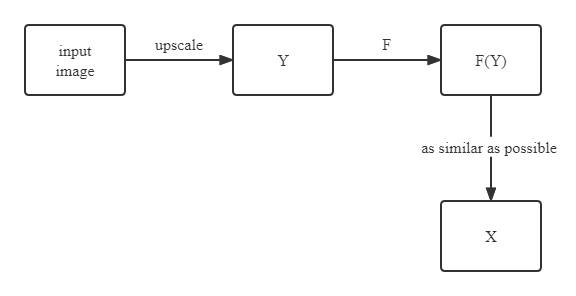
\includegraphics[scale=0.5]{figure/p1.png}
  \caption{流程图}
  \label{fig:p1}
\end{figure}

我们想要学习的这个函数F,其实可以分解成以下三部分操作:


1.Patch extraction and representation:从Y中提取出patch,然后将每个patch映射成一个高维向量,并且这些向量可以组成一个featuremap,这个操作等同于使用带有偏置的卷积核在图片上进行卷积运算,我们可以写成:
$$F_1(Y)=max(0,W_1\ast Y+B_1)$$
其中W1、B1分别表示为卷积核和偏置,*表示卷积运算;W1对应于n1个大小为c×f1×f1的卷积核(c表示输入图片的通道数)。

2.Non-linear mapping:将上一步得到的高维向量经过非线性变换转换为另一个高维向量,这些高维向量也能得到一个featuremap,这个操作对应于使用n2个大小为1×1的卷积核进行运算,当然卷积核的大小是可以改变的,使用更大的卷积核会有更好的泛化效果,我们可以写成:
$$F_2(Y)=max(0,W_2\ast F_1(Y)+B_2)$$
其中W2对应于n2个大小为n1×f2×f2的卷积核。虽然增加更多的卷积层能增加非线性,但是会使得模型复杂度增加,从而需要更多的训练时间。

3.Reconstruction:将上一步生成的高维向量合成最终的高分辨率图片输出,这个操作可以看成在featuremap上使用预先定义的卷积核进行averaging的过程,这是一个线性过程:
$$F(Y)=W_3\ast F_2(Y)+B_3$$
其中W3对应于c个大小为n2×f3×f3的卷积核。

以上的操作如图\ref{fig:p2}所示。

\begin{figure}[H]
  \centering
  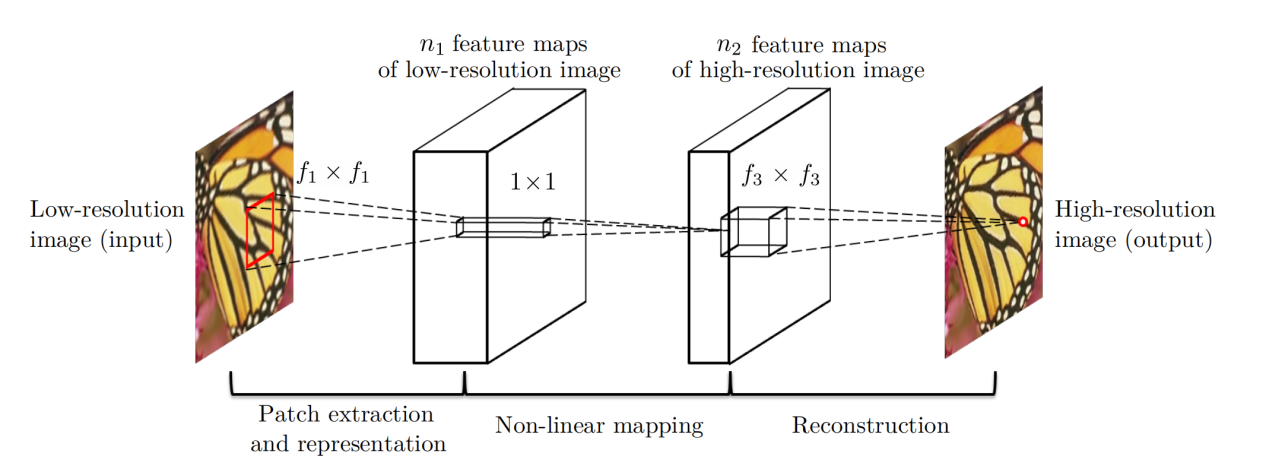
\includegraphics[scale=0.8]{figure/p2.png}
  \caption{学习模型}
  \label{fig:p2}
\end{figure}

\subsection{和基于稀疏编码的SR方法的关系}
传统的基于稀疏编码的SR方法可以被看成一个卷积神经网络,如图\ref{fig:p3}所示:
\begin{figure}[H]
  \centering
  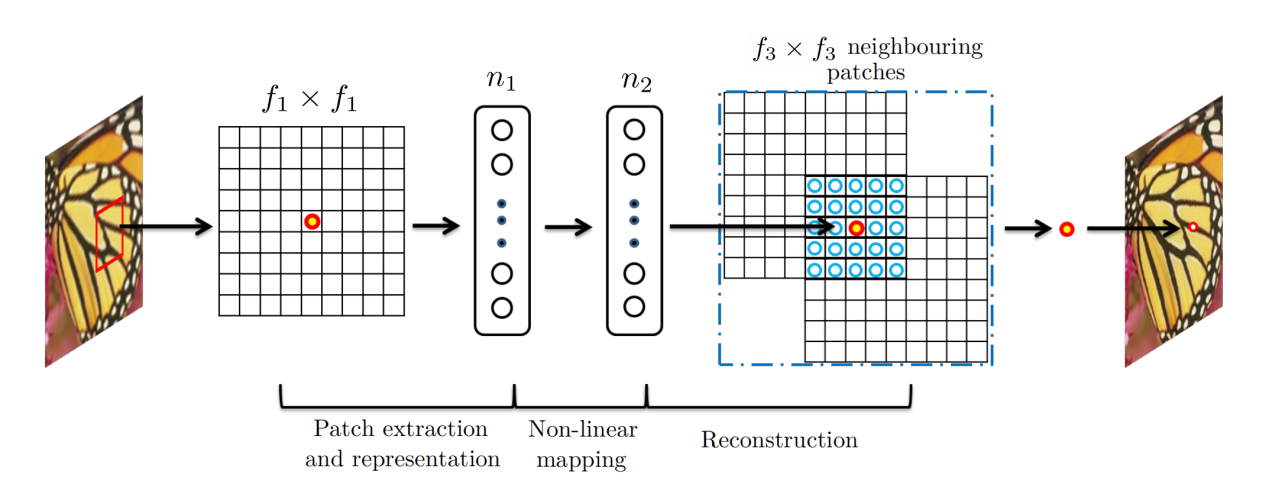
\includegraphics[scale=0.8]{figure/p3.png}
  \caption{卷积神经网络}
  \label{fig:p3}
\end{figure}
在基于稀疏编码的SR方法模型中,我们可以把f1×f1低分辨率的patch看成是从输入图片提取出来的,然后稀疏编码求解程序将patch投影到一个字典上,如果这个字典的大小为n1,那么相当于在输入图片上使用n1个大小f1×f1的卷积核进行卷积运算,如上图的左半部分所示。稀疏编码求解程序会迭代的处理n1维度的向量,从而得到一个n2维度的向量,一般来说n1、n2是相等的,这个时候稀疏编码求解程序起的作用就是一个大小为1×1的非线性映射运算符,如上图的中间部分所示。然后再对n2维度的向量投影到另一个字典空间目的是产生高分辨率的patch,重叠部分的patch会进行平均操作,如上图的右半部分所示。

在SRCNN中,以上的低分辨率字典、高分辨率字典、非线性映射、减去均值和平均化的操作都包括在需要优化的卷积核里了,所以说该模型是一个包括所有操作的端到端的映射。而且之所以SRCNN的表现更好是因为SRCNN使用更多的像素信息用于图像重构。例如当我们设置f1=9,f2=1,f3=5,n1=64,n2=32时,高分辨率像素使用了(9+5-1)\^{}2=169个像素的信息,而传统的方法只使用了(5+5-1)\^{}2=81个像素的信息。

\subsection{训练}

该模型的参数有:W1,W2,W3,B1,B2,B3。给定一组高分辨率图片Xi以及对应低分辨率图片Yi,我们使用MSE作为损失函数:
$$L(\varnothing)=\frac1n\sum_{i=1}^n\left\|F(Y_i;\varnothing)-X_i\right\|^2$$

其中n表示训练样本的数量,使用MSE作为损失函数会使得PSNR值变得很高,损失函数使用SGD进行优化,参数的更新过程如下所示:
$$\triangle_{i+1}=0.9\cdot\triangle_i-\mu\cdot\frac{\partial L}{\partial W_i^l},W_{i+1}^l=W_i^l+\triangle_{i+1}$$
参数Wi使用均值为0标准差为0.001的高斯分布进行初始化,参数Bi初始化为0,前两层的学习率为10\^{}-4,最后一层的学习率为10\^{}-5,而且作者发现在最后一层使用小的学习率对于SRCNN收敛很重要。为了避免在训练时边界影响,所有CNN都采用no padding的策略。


\section{实验结果}
\subsection{训练集大小对实验结果的影响}
使用大型的训练集可能对SRCNN的表现有提升,但是训练集大小的影响不大,不像如分类问题那么明显。
\subsection{SR中已学习的卷积核}
第一层的featuremap中包括不同的结构,例如不同方向上的边缘;第二层主要是光照强度的不同。
\subsection{模型大小和模型表现的折衷}
\subsubsection{卷积核的数量}
通过增加卷积核的数量能得到更好的性能,但是卷积核越多,图像重构的时间越长。
\subsubsection{卷积核大小}
适当的增大卷积核大小能获得更多的结构信息,所以会得到更好的结果。增大第二层卷积核的大小能显著提升性能,这说明利用周围的信息在映射阶段是有益的;但是增大第二层卷积核大小会使得模型复杂度、以及降低了部署的时间。
\subsubsection{层的数量}
四层网络比三层网络的收敛速度慢,但是给定足够的时间,四层网络最后也会追上三层网络的。但是并不像图像分类问题上网络深度越深效果越好,SR问题并不能看出网络深度对网络表现的影响,而且随着网络深度的增加可能还会导致性能的下降。

导致以上结论的原因可能是SRCNN没有池化层和全连接层,所以它对初始化参数和学习率很敏感。当模型层数增加时,我们很难保证找到一组合适的学习率使得其收敛,即使模型收敛了,也可能陷入一个不好的局部最小值,并且经过足够的训练时间,已学习的卷积核的多样性会变少。而且在图像分类领域,不适当的增加模型深度也会使得准确率的下降或退化。

\section{总结}
作者提出了基于稀疏编码的卷积方法,并将其实现为一个深度神经网络SRCNN,能够学习端到端的低分辨率图片到高分辨率图片的映射,而且这是个轻量级的结构,有着超越其他state-of-art方法的表现。


\chapter{VDSR}
\section{摘要}

作者提出了一种高精度单幅图像超分辨率方法。该方法使用了一个受VGG网络启发的深度进化网络,用于图像网络分类。增加网络深度会显著提高准确性,最终模型使用20个重量层。通过在深层网络结构中多次级联小过滤器,以有效的方式利用大图像区域上的上下文信息。然而,对于非常深的网络,收敛速度成为训练中的一个关键问题。作者提议一个简单而有效的训练程序,只学习残差,并使用极高的学习率(比SRCNN高104倍)由可调梯度削波启用。

%——————————————————————————————————————
\section{介绍}

单幅图像超分辨率(SISR):解决在给定低分辨率(LR)图像的情况下生成高分辨率(HR)图像的问题。

SISR广泛用于计算机视觉应用,早期方法包括插值,如双三次插值和Lanczos重采样利用统计图像先验的更强大的方法或内部补丁复发。

目前,学习方法被广泛用于模拟从LR到HR面片的映射。邻居嵌入方法插值面片子空间。稀疏编码方法使用基于稀疏信号表示的学习紧凑字典。最近,兰登森林和卷积神经网络(CNN)在准确性方面也有了很大的提高。

SRCNN成功地将深度学习技术引入到超分辨率问题中,但在三个方面存在局限性:
\begin{itemize}
  \item 它依赖于小图像区域的上下文;
  \item 训练收敛太慢;
  \item 网络只对单一尺度起作用。
\end{itemize}

作者提出了一个基于非常深的卷积网络的高精度随机共振方法。如果使用小的学习率,非常深的网络收敛太慢。如果使用高学习率提高收敛率会导致梯度爆炸,于是用剩余学习和梯度削波来解决这个问题。此外,作者扩展了工作处理单一网络中的多尺度随机共振问题。

%——————————————————————————————————————
\section{相关工作}

SRCNN是一种具有代表性的基于深度学习的SR方法。因此,让我们用我们提出的方法进行分析和比较。

\subsection{图像超分辨率卷积网络}

SRCNN模型由三层组成:面片提取/表示、非线性映射和重建。

作者认为增加深度可以显著提高性能。使用了20个配重层(每层3 × 3),深度关系网(20vs3),用于重建的信息更大(41 × 41对13 × 13)。

Training SRCNN直接建模高分辨率图像。SRCNN的两个目的:将输入传送到末端层和重构残差。由于网络直接对残差图像进行建模,可以以更高的精度实现更快的收敛。

Scale SRCNN针对单个比例因子进行训练,仅与指定的比例一起工作。为了处理多尺度随机共振(可能包括分数因子),需要为每个感兴趣的尺度构建单独的单尺度随机共振系统。

作者为了使网络符合各种场景,设计并训练了一个单一网络来有效地处理多尺度随机共振问题。

细节部分,输出图像与输入图像具有相同的大小,通过在训练期间每层填充零,而来自SRCNN的输出小于输入。简单地对所有层使用相同的学习速率,而SRCNN对不同层使用不同的学习速率,以实现稳定的收敛。

\section{推荐的方法}
\subsection{推荐的网络}

超分辨率图像重建,使用非常深度卷积网络,配置如图所示。

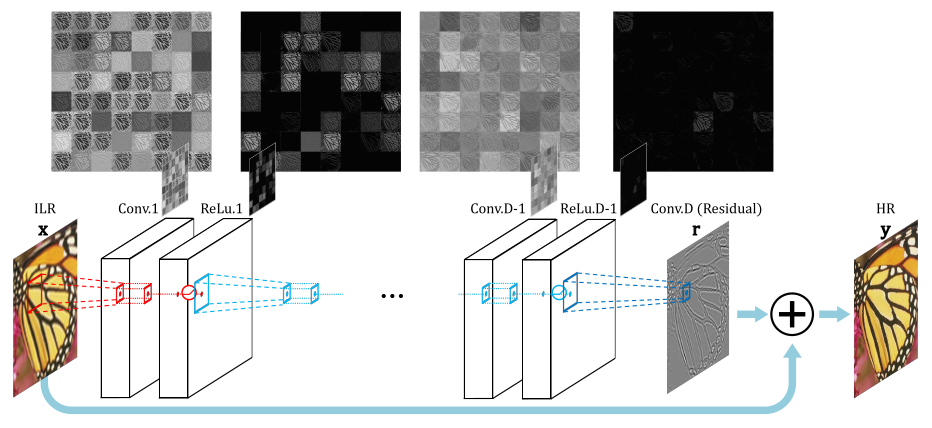
\includegraphics[width=\textwidth]{figure/peizhi.png}

基于CNN的方法可以从超分辨率方法中获益,因为超分辨率方法中经常使用对图像细节建模的方法。

使用非常深度网络来预测密集输出的一个问题:每次应用卷积运算时特征图的大小变小了。

如果所需的环绕区域非常大,这种方法就无效。裁剪后,最终图像太小,视觉效果不佳。为了解决这个问题,在卷积之前填充零以保持所有特征图的大小(包括输出)相同。

一旦图像细节被预测,它们被添加回输入ILR图像以给出最终图像(HR)。

\subsection{训练}
描述最小化的目标,以便找到模型的最佳参数:

设x表示插值的低分辨率图像,y表示高分辨率图像,给定训练数据集$\{x^{(i)},y^{(i)}\}$,目的是预测$\hat{y}=f(x)$,其中$\hat{y}$是目标HR图像的估计值。要使平方误差$\frac{1}{2}||y-f(x)||^2$最小化。

Residual-Learning 利用剩余学习来解决渐晕/梯度爆炸问题问题。定义残差图像$r=y-x$,要去预测残差图像,损失函数变为$\frac{1}{2}||r-f(x)||^2$,$f(x)$为网络预测。

High Learning Rates for Very Deep Networks 在真实的时间限制下,深层模型可能存在无法收敛的问题。学习率高,以促进训练是常规策略。但是简单地将学习速率设置得很高也会导致梯度消失/爆炸。为此,在抑制爆炸梯度的同时,采用可调的梯度削波来最大限度地提高速度。

Adjustable Gradient Clipping 可调梯度裁剪的使用仅限于训练CNN。其中一个常用的策略是对个体进行裁剪预定义范围$[-\theta,\theta]$的梯度。随机梯度下降常用于训练,学习率乘以调整步长。如果使用高学习率,很可能将θ调整为较小,以避免在高学习率状态下爆发梯度。但是,随着学习率被退火以变得更小,有效梯度(梯度乘以学习率)接近零,并且如果学习率以几何方式降低,则训练可能需要指数多次迭代才能收敛。为了达到最快的收敛速度,我们剪切梯度$[-\frac{\theta}{\gamma},\frac{\theta}{\gamma}]$,$\gamma$表示当前学习速率。

Multi-Scale 使用更多的参数来定义网络。考虑到经常使用分数比例因子,需要一种经济的方法来存储和检索网络。为此,训练了一个多尺度模型。使用这种方法,参数在所有预定义的比例因子之间共享。

残差和非残差网络的性能表(PSNR)如图:

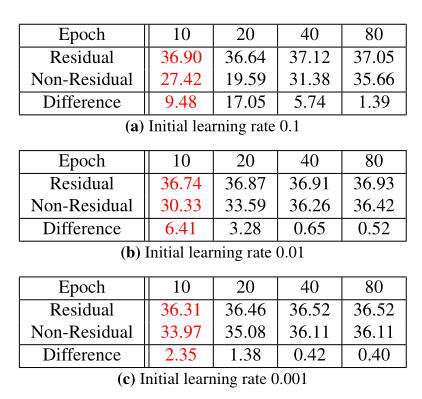
\includegraphics[width=0.5\textwidth]{figure/cancha.png}

\section{了解性质}
讨论了作者提出的方法的三个性质:

\begin{itemize}
  \item 学习深度越深越好;
  \item 该剩余学习网络可以比标准的CNN快得多且大大提高了性能;
  \item 该网络是适用于多种规模的单一模型。
\end{itemize}

通过实验证明,非常深的网络可以显著提高随机共振的性能。训练和测试深度范围从5到20的网络(仅计算权重层,不包括非线性层),结果如图:

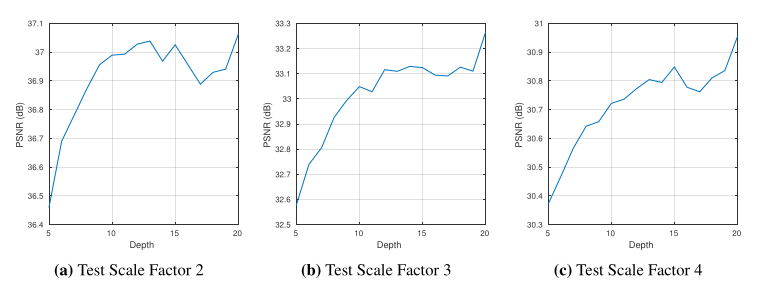
\includegraphics[width=\textwidth]{figure/depth.png}

使用深度10(权重层)和比例因子2。不同学习率下的性能曲线如图:

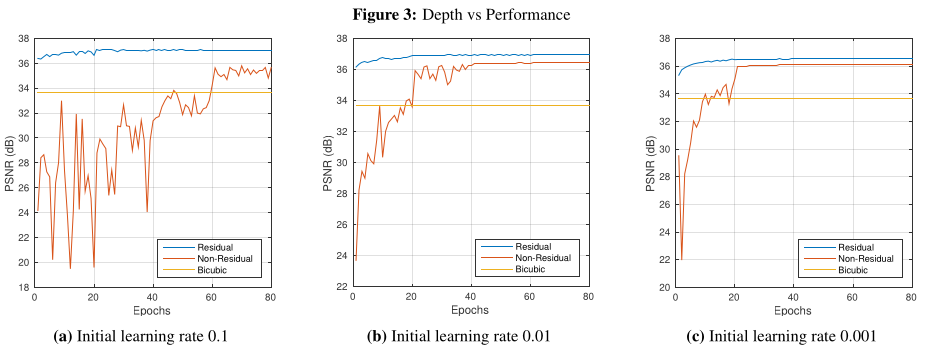
\includegraphics[width=\textwidth]{figure/rate.png}
在收敛时,剩余网络表现出优越的性能。

%——————————————————————————————————————
\section{实验结果}
描述用于训练和测试我们方法的数据集后,给出训练所需的参数,将该方法与几种最先进的SISR方法进行了比较。

\subsection{用于训练和测试的数据集}
作者采用了参考文献中使用的各种不同类型具有挑战性的数据集。

\subsection{训练参数}
使用深度为20的网络。训练使用大小为64的batch size。动量和重量衰减参数设置为0.9和0.0001。在80个时期内训练所有实验,9960次迭代。学习率最初设置为0.1,每20个时期减少10倍。总体而言,学习率降低了3倍,并且在80个周期后停止学习。

\subsection{基准测试}
遵循公开可用的黄等人的框架,该框架将双三次插值应用于图像的颜色分量,裁剪图像边界附近的像素。

\subsection{与最先进方法的比较}
分为定量和定性的比较,与A+, RFL, SelfEx和SRCNN进行比较。

下表是定量比较的结果:

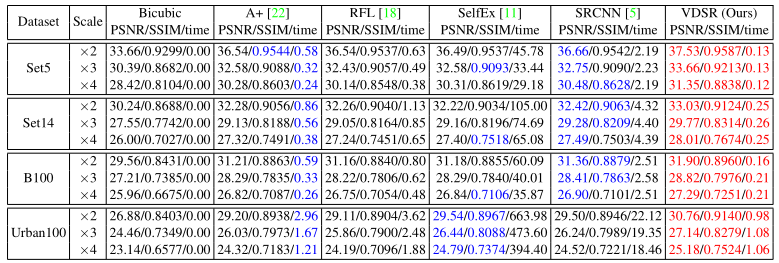
\includegraphics[width=\textwidth]{figure/dingliang.png}

可见该方法优于以前所有方法并且相对较快。

下面两图是与性能最好的方法比较。第一张图中,只有该方法完美地重构了中间的线。第二张图中,轮廓在该方法中是清晰和生动的,而在其他方法中它们是严重模糊或失真的。

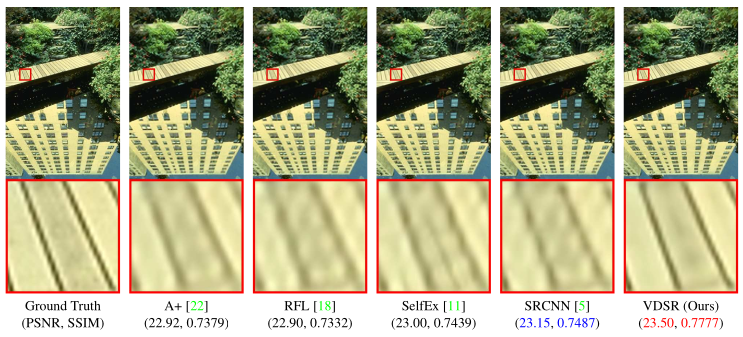
\includegraphics[width=\textwidth]{figure/6.png}

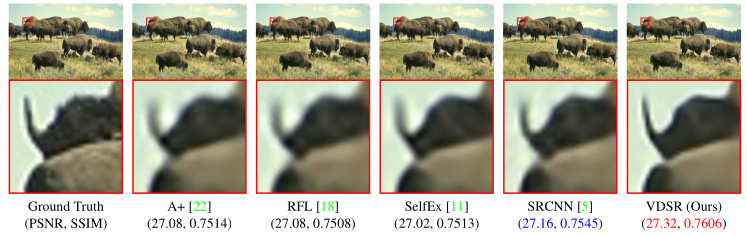
\includegraphics[width=\textwidth]{figure/7.png}

\subsection{结论}
作者提出了一个使用非常深度的网络来超分辨率的方法。由于收敛速度慢,训练非常深的网络很困难,于是使用剩余学习和极高的学习率来快速优化非常深度的网络。收敛速度被最大化,并且使用梯度裁剪来保证训练的稳定性。已经证明了该方法在基准图像上比现有的方法有更大的优势。今后该方法可能会应用于其他图像恢复问题,如去噪和压缩伪像消除。


\chapter{SRGAN}
\section{摘要}
从低分辨率图像还原高分辨率图像的困难任务被称为超分辨率,其受到了计算机视觉研究领域的广泛关注,具有广泛的研究范围。

尽管使用更快,更深层次卷积神经网络在单图像超分辨率上的准确性和速度取得了突破,但是一个核心问题在很大程度上仍然没有解决:
当我们在进行大比例上采样时,如何恢复更精细的纹理细节?这种基于优化的超分辨率方法主要由目标函数的选择驱动。
最近的工作主要集中于最小化重建错误平均值平方。
这样带来的结果虽然有高峰值信噪比,但通常缺乏高频细节,在感官上令人不满意:它们没有高分辨率所对应的高保真度。

在本文中,我们提出了SRGAN,图像超分辨率(SR)的生成对抗网络(GAN)。
据我们所知,这是第一个能够推断出真实自然的4倍超分辨率图像的框架。为了实现这一点,我们提出了一个由对抗损失和内容损失组成的感知损失函数。
对抗性损失器使用一个经过训练的分类器网络来区分超分辨率图像和原始真实图像,以将结果导向自然图像处理器。
此外,我们使用由感知相似性而不是像素相似性激活的内容损失器。

在公共测试集数据中,我们的深层残差网络能够从重度下采样的图像中修复真实材质。
在MOS测试中,使用SRGAN获得的高分辨率图像比任何其他图像超分辨率方法都要接近原始图像。

\section{介绍}
在本文中,我们提出了一个超分辨率生成对抗网络 SRGAN,其中我们采用了一个具有跳跃连接和偏离MSE的深度残差网络 ResNet 作为唯一优化目标。
与之前的工作不同的是,我们使用 VGG 网络的高级特征图,结合了一个识别器来定义一种新的感知损失,该识别器激励了难以从高分辨率图像 HR 中分离出来的特征。

这里我们将重点讨论单图像超分辨率 SISR,不再进一步讨论从多幅图像恢复 HR 图像的方法。

相关工作:
\begin{itemize}
  \item 基于预测的过滤方法,速度快但是会生成过于光滑的纹理
  \item 建立低分辨率和高分辨率图像信息之间的复杂映射,通常依赖于训练数据
  \item 将基于梯度轮廓先验的边缘重定向 SR 算法和基于学习的优点相结合,在避免边缘伪影的同时重建真实的纹理细节
  \item 邻域嵌入方法通过在低维簇中寻找相似的LR训练快,并结合它们对应的HR块进行重建
  \item 基于卷积神经网络 CNN 的SR算法表现出了优异的性能
\end{itemize}

算法表现出了优异的性能。Wang et al基于学习的迭代收缩和阈值算法LISTA在前馈网络结构中编码了一个稀疏表示。Dong等人使用双三次插值对输入图像进行上采样,并对三层深度全卷积网络进行端到端训练,以实现最先进的SR性能。随后,研究表明,让网络直接学习缩放滤波器可以进一步提高精度和速度。Kim等人利用他们的深度递归卷枳网络DRCN,提出了一种高性能的架构,允许长范围像素依赖,同时保持模型参数的数量很小。与我们的论文特别相关的是Johnson等人和Bruna等人的工作,他们依靠更接近感知相似性的损失函数恢复在视觉上更有说服力的HR图像。

\subsection{卷积神经网络的设计}
研究表明,更深层次的网络架构可能很难训练,但有可能大幅提高网络的准确性,因为它们允许非常复杂的建模映射。
为了有效地训练这些更深层次的网络结构,批处理归一化经常被用来抵消内部协变最移位。
更深层次的网络架构也被证明可以提高SISR的性能。另一个简化深度cnn训练的强大设计选择是最近引入的残差块和跳跃连接的概念。跳跃连接减轻了网络体系结构建模身份映射的负担,这在本质上是微不足道的,然而,用卷积核表示可能不是微不足道的。
在SISR的背景下,学习缩放滤波器在精度和速度方面也是有益的。这是对Dong等人的改进, 在将图像输入CNN之前,使用双三次插值来扩大LR的观察值。

\subsection{损失函数}
像素级损失函数(如MSE)处理恢复丢失的高频细节(如纹理)具有固有的不确定性:最小化MSE以寻找合理解,这些解通常过于光滑,因此具有较差的观感。
使用在神经网络特征空间计 欧式距离的损失函数,并结合对抗性训练。结果表明,能生成视觉上更优越的图像,并可用于解决解码非线性特征表示的病态问题。与这项工作类似,使用从预先训练的VGG网络提取的特征,而不是简单的像索级误差评估,能获得在观感上超分辨率和风格都更令人信服的结果。

\subsection{贡献}
在这篇文章中,我们描述了第一个非常深入的 ResNet架构。我们的主要贡献是:
\begin{itemize}
  \item 我们通过PSNR和结构相似度SSIM来测最高缩放因子(4X)的图像SR,并采用针对MSE优化的16块深度 ResNet (SRResNet)
  \item 我们提出了 SRGAN,这是一个基于GAN的网络,针对新的感知损失进行了优化。在这里,我们将基于MSE的内容损失替换为在VGG网络的特征映射上计算的损失,它对像素空间的变化更不稳定
  \item 我们通过对来自三个公共基准数据集的图像进行广泛的平均意见评分MOS测试确认,SRGAN在很大程度上是一种新的技术,用于建立具有高缩放因子(4X)的逼真SR图像
\end{itemize}

\section{方法}
在 SISR 中,我们从低分辨率的输入图像 $I^{LR}$ 生成超分辨率的图像 $I^{SR}$,$I^{LR}$是高分辨率图像$I^{HR}$的低分辨率版本,高分辨率图像只在训练期间可用。
在训练期间,$I^{LR}$为使用比例因子为r进行的对$I^{HR}$高斯滤波下采样操作获得的图像。
对于一个有着 $C$个颜色通道的图像,我们使用大小为 $W × H × C$的实张量描述$I^{LR}$,使用大小为 $rW × rH × C$的实张量描述$I^{HR}$和$I^{SR}$

我们的最终目标是训练一个生成函数G,它可以对LR输入图像预测对应的HR图像。对此,我们训练了一个参数化$\theta_G$的前馈 CNN $G_{\theta_G}$生成网络,
$\theta_G = \{W_{1:L};b_{1:L}\}$表示 $L$层网络的权重和偏差,是通过对SR的特定损失函数$l^{SR}$进行优化得到。
对于训练图片 $I^{HR}_n, n = 1, ..., N$及相应的$I^{LR}_n, n = 1, ..., N$,我们求解:
\begin{equation}
  \hat{\theta}_G = arg\ \mathop{min}\limits_{\theta_G} \frac{1}{N} \sum_{n = 1}^{N} l^{SR}(G_{\theta_G}(I_n^{LR}), I_n^{HR})\label{eq:1}
\end{equation}
我们将专门设计几个相异模型的损失函数的加权组合作为新的感知损失模型$l^{SR}$。

\subsection{对抗网络架构}
我们进一步定义了一个分类器网络 $D_{\theta_D}$,使用$G{\theta_G}$以一种交替的方式来优化它,来解决对抗的 min-max问题:
\begin{equation}
  \mathop{min}\limits_{\theta_G} \mathop{max}\limits_{\theta_D} \mathbb{E}_{I^{HR} \sim p_{train}(I^{HR})}[logD_{\theta_D}(I^{HR})] + \mathbb{E}_{I^{LR} \sim p_G(I^{LR})}[log(1 - D_{\theta_D}(G_{\theta_G}(I^{LR})))]\label{eq:2}
\end{equation}
这个公式的一般想法是,它允许训练生成模型 G,目的可能是欺骗可微分类器 D,该分类器被训练来区分超分辨率图像和真实图像。通过这种方法,我们的生成器可以学习创建与真实图像高度相似的解,因此很难通过D进行分类。
生成网络 G 的核心使用两个卷积层其中包含 $3 × 3$ 内核和 64 个 特征映射,然后使用batch标准化层和ParametricReLU作为激活函数。通过两个经过训练的亚像素卷积层来提高输入图像的分辨率。

为了从生成的SR样本中区分真实的HR图像,我们训练了一个分类器网络。LeakyReLU 激活 ($\alpha = 0.2$),避免整个网络的最大池化。训练判别器网络来求解方程 \ref{eq:2} 中的最大化问题。它包含8个卷积层,每层$3 × 3$个卷积核,与VGG网络一样,从64个核增加到512个核,增加了2倍。当特征数增加一倍时,采用跨步卷积来降低图像分辨率。在生成的512个特征图之后, 再经过两个密集层和一个最终的sigmoid激活函数来获得样本分类的概率。

\subsection{感知损失函数}
我们感知损失函数的定义$l^{SR}$对生成网络的性能至关重要。而$l^{SR}$通常基于MSE建模,我们改进了Johnson和Bruna等人的成果,并设计了一个损失函数, 根据感知相关特征评估解决方案。我们将感知损失表示为内容损失$l_X^{SR}$和对抗损失如下:
\begin{equation}
  l^{SR} = \underbrace{\underbrace{l_X^{SR}}_{content\ loss} + \underbrace{10^{-3} l_{Gen}^{SR}}_{adversarial\ loss}}_{perceptual\ loss\ (for\ VGG\ based\ content\ losses)}\label{eq:3}
\end{equation}

\subsubsection{内容损失}
像素级MSE损失函数的计算方法:
\begin{equation}
  l_{MSE}^{SR} = \frac{1}{r^2WH}\sum_{x = 1}^{rW}\sum_{y = 1}^{rH}(I_{x, y}^{HR} - G_{\theta_G}(I^{LR})_{x, y})^2\label{eq:4}
\end{equation}

这是图像SR最广泛使用的优化目标,许多最先进的方法都依赖于此。然而,在获得特别高的PSNR的同时,MSE优化问题的解决方案往往缺乏高频率内容,导致过于光滑的纹理。

我们不依赖像素级损失,而是基于 Gatys、 Bruna和Johnson等人的思想,并使用更接近感知相似性的损失函数。我们基于 Simonyan和Zisserman描述的预训练19层VGG网络的ReLU激活层来定义 VGG损失。用$\phi_{i, j}$我们表示VGG19网络中第$i$个 maxpooling层之前的第$j$个卷积(激活后)得到的特征映射,然后我们将VGG损失定义为由构图像G 的特征$G_{\theta_G}(I^{LR})$和原始图像$I^{LR}$表示之间的欧氏距离
\begin{equation}
  l_{VGG / i, j}^{SR} = \frac{1}{W_{i, j}H_{i, j}}\sum_{x = 1}^{W_{i, j}}\sum_{y = 1}^{H_{i, j}}(\phi_{i, j}(I^{HR})_{x, y} - \phi_{i, j}(G_{\theta_G}(I^{LR}))_{x, y})^2\label{eq:5}
\end{equation}
这里 $W_{i, j}$和$H_{i, j}$描述了VGG网络中各自特征图的维度。

\subsubsection{对抗损失}
除了到目前为止所描述的内容损失,我们还将GAN的生成成分添加到感知损失中。这鼓励我们的网络倾向于通过尝试得到欺骗分类器的解决方案。生成损失$l_{Gen}^{SR}$定义基于分类器对于所有训练样本的概率$D_{\theta_D}(G_{\theta_G}(I^{LR}))$为:
\begin{equation}
  l_{Gen}^{SR} = \sum_{n = 1}^{N} -\log{D_{\theta_D}(G_{\theta_G}(I^{LR}))}\label{eq:6}
\end{equation}
这里的$D_{\theta_D}(G_{\theta_G}(I^{LR}))$表示重构图像$G_{\theta_G(I^{LR})}$是自然 HR 图像的概率。为了更好的梯度行为,我们选择最小化$-\log{D_{\theta_D}(G_{\theta_G}(I^{LR}))}$而不是$\log{[1 - D_{\theta_D}(G_{\theta_G}(I^{LR}))]}$

\section{实验总结}
我们通过MOS测试证实了 SRGAN优越的感知性能。我们进一步表明,标准的量化措施,如PSNR和SSIM,无法捕获和准确评估与人类视觉系统相关的图像质量。这项工作的重点是超分辨率图像的感知质量,而不是计算效率。与Shi等人的模型相比,该模型没有对视频 SR进行实时优化。然而,对网络架构的初步实验表明,浅层网络有可能在质量表现上略有下降的情况下提供非常有效的替代方案。与Dong等人的研究相比,我们发现更深层次的网络架构是有益的。我们推测ResNet 设计对更深层次网络的性能有很大的影响。

\section{结论}
我们描述了一个深度残差网络SRResNet,当使用广泛使用的PSNR公共数据集时,它达到了一个新的里程碑。我们也强调了PSNR的一些局限性,提出了SPGAN算法,
该算法通过训练GAN来增强内容损失函数的对抗性损失,通过大量的MOS测试,我们已经证实,在较大的缩放因子(4X)下,SRGAN重建比使用最先进的其他参考方法得到的重建图像在很大程度上更加逼真。
% 参考文献\cite{adams1995hitchhiker}\cite{shin2016deep}

% \newpage
% \bibliographystyle{plain}
% \bibliography{reference}
\end{document}
